\documentclass{standalone}
\usepackage{tikz}

\begin{document}
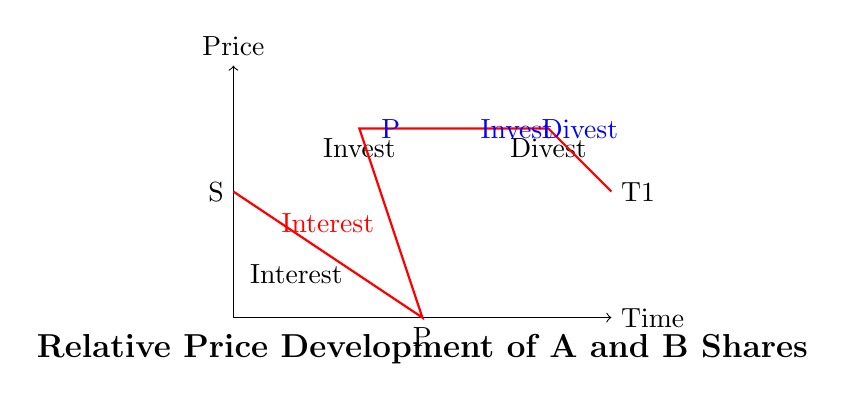
\begin{tikzpicture}[scale=0.8]
    % Whiteboard background
    \fill[white] (0,0) rectangle (6,4);

    % Axes
    \draw[->] (0,0) -- (6,0) node[right] {Time};
    \draw[->] (0,0) -- (0,4) node[above] {Price};

    % Points and labels
    \coordinate[label=left:S] (S) at (0,2);
    \coordinate[label=right:T1] (T1) at (6,2);
    \coordinate[label=below:P] (P) at (3,0);
    \coordinate[label=below:Interest] (Interest) at (1,1);
    \coordinate[label=below:Invest] (Invest) at (2,3);
    \coordinate[label=below:Divest] (Divest) at (5,3);

    % Line connecting points
    \draw[thick, red] (S) -- (P) -- (Invest) -- (Divest) -- (T1);

    % Annotations
    \node at (1.5,1.5) [red] {Interest};
    \node at (2.5,3) [blue] {P};
    \node at (4.5,3) [blue] {Invest};
    \node at (5.5,3) [blue] {Divest};

    % Title
    \node at (3,-0.5) [font=\large\bfseries] {Relative Price Development of A and B Shares};
\end{tikzpicture}
\end{document}